\documentclass{standalone}
\usepackage{tikz}
\usetikzlibrary{patterns}
\usetikzlibrary{positioning}
\usetikzlibrary{patterns, positioning}
\usetikzlibrary{shapes.misc}
\usepackage[outline]{contour}
\contourlength{1.5pt} 
\usetikzlibrary{calc}
        \usepackage{relsize}
        \tikzset{fontscale/.style = {font=\relsize{#1}}}

\begin{document}
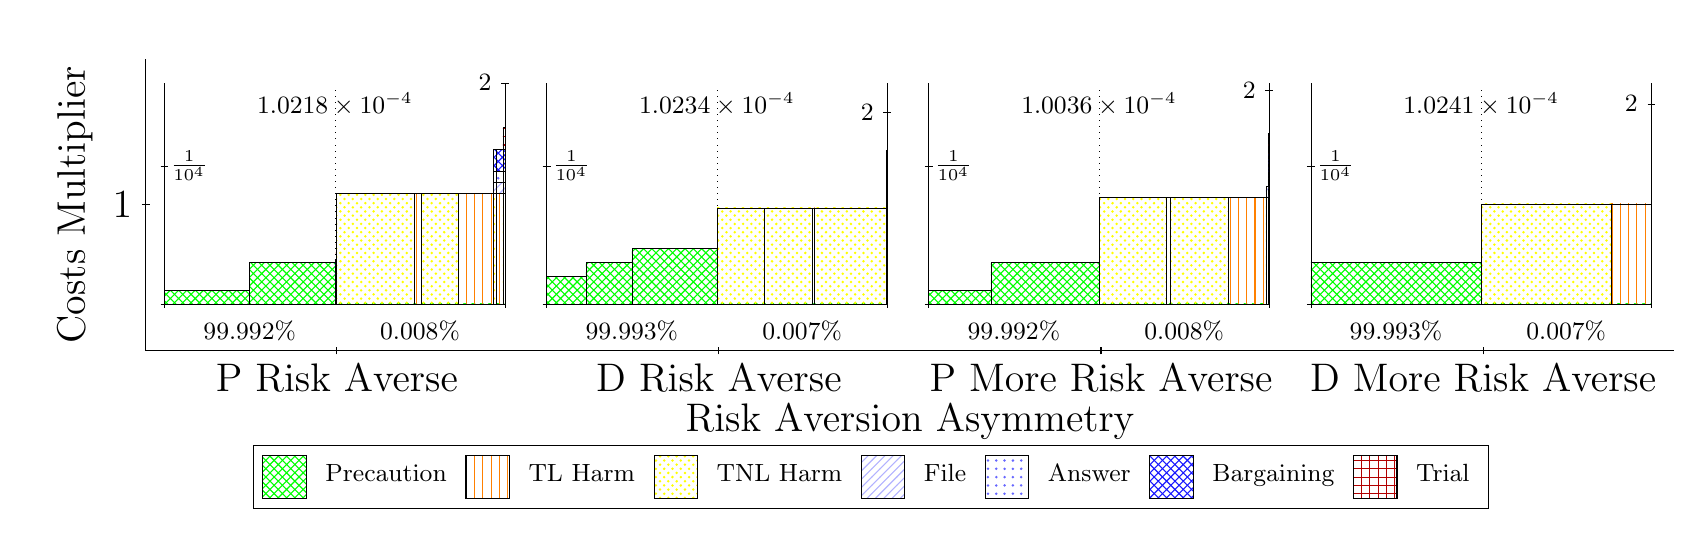
\begin{tikzpicture}
\clip(-0.5,-1.1) rectangle +(20.91,6.2);
\draw[black] (1,1) -- (1,4.7);
\node[rotate=90, fontscale=2, anchor=center] at (0.1, 2.85) {Costs Multiplier};
\draw[black] (0.95,2.85) -- (1.05,2.85);
\node[fontscale=2, anchor=east] at (0.95, 2.85) {1};

\draw[black] (1,1) -- (20.41,1);
\node[fontscale=2, anchor=center] at (10.705, 0.1) {Risk Aversion Asymmetry};
\draw[black] (3.4263,0.95) -- (3.4263,1.05);
\node[fontscale=2, anchor=north] at (3.4263, 0.95) {P Risk Averse};
\draw[black] (8.2788,0.95) -- (8.2788,1.05);
\node[fontscale=2, anchor=north] at (8.2788, 0.95) {D Risk Averse};
\draw[black] (13.131,0.95) -- (13.131,1.05);
\node[fontscale=2, anchor=north] at (13.131, 0.95) {P More Risk Averse};
\draw[black] (17.984,0.95) -- (17.984,1.05);
\node[fontscale=2, anchor=north] at (17.984, 0.95) {D More Risk Averse};


\draw[pattern=crosshatch, pattern color=green,draw=black,very thin] (1.2381,1.592) rectangle (2.3197,1.7674);
\draw[pattern=crosshatch, pattern color=green,draw=black,very thin] (2.3197,1.592) rectangle (3.4013,2.1181);
\draw[pattern=crosshatch, pattern color=green,draw=black,very thin] (3.4013,1.592) rectangle (3.415,1.592);
\draw[pattern=north east lines, pattern color=blue!30,draw=black,very thin] (3.4013,1.592) rectangle (3.415,1.7324);
\draw[pattern=dots,  pattern color=blue!60,draw=black,very thin] (3.4013,1.7324) rectangle (3.415,1.8728);
\draw[pattern=crosshatch,      pattern color=blue!90,draw=black,very thin] (3.4013,1.8728) rectangle (3.415,2.1536);
\draw[pattern=crosshatch, pattern color=green,draw=black,very thin] (3.415,1.592) rectangle (3.4184,1.592);
\draw[pattern=north east lines, pattern color=blue!30,draw=black,very thin] (3.415,1.592) rectangle (3.4184,1.7324);
\draw[pattern=dots,  pattern color=blue!60,draw=black,very thin] (3.415,1.7324) rectangle (3.4184,1.8728);
\draw[pattern=crosshatch,      pattern color=blue!90,draw=black,very thin] (3.415,1.8728) rectangle (3.4184,2.1536);
\draw[pattern=grid,            pattern color=red!70!black,draw=black,very thin] (3.415,2.1536) rectangle (3.4184,2.4344);
\draw[pattern=crosshatch, pattern color=green,draw=black,very thin] (3.4184,1.592) rectangle (4.4077,1.592);
\draw[pattern=crosshatch dots, pattern color=yellow,draw=black,very thin] (3.4184,1.592) rectangle (4.4077,2.996);
\draw[pattern=crosshatch, pattern color=green,draw=black,very thin] (4.4077,1.592) rectangle (4.503,1.592);
\draw[pattern=vertical lines, pattern color=orange,draw=black,very thin] (4.4077,1.592) rectangle (4.503,2.996);
\draw[pattern=crosshatch, pattern color=green,draw=black,very thin] (4.503,1.592) rectangle (4.9676,1.592);
\draw[pattern=crosshatch dots, pattern color=yellow,draw=black,very thin] (4.503,1.592) rectangle (4.9676,2.996);
\draw[pattern=crosshatch, pattern color=green,draw=black,very thin] (4.9676,1.592) rectangle (5.4116,1.592);
\draw[pattern=vertical lines, pattern color=orange,draw=black,very thin] (4.9676,1.592) rectangle (5.4116,2.996);
\draw[pattern=crosshatch, pattern color=green,draw=black,very thin] (5.4116,1.592) rectangle (5.4555,1.592);
\draw[pattern=crosshatch dots, pattern color=yellow,draw=black,very thin] (5.4116,1.592) rectangle (5.4555,2.996);
\draw[pattern=north east lines, pattern color=blue!30,draw=black,very thin] (5.4116,2.996) rectangle (5.4555,3.1364);
\draw[pattern=dots,  pattern color=blue!60,draw=black,very thin] (5.4116,3.1364) rectangle (5.4555,3.2768);
\draw[pattern=crosshatch,      pattern color=blue!90,draw=black,very thin] (5.4116,3.2768) rectangle (5.4555,3.5576);
\draw[pattern=crosshatch, pattern color=green,draw=black,very thin] (5.4555,1.592) rectangle (5.5338,1.592);
\draw[pattern=vertical lines, pattern color=orange,draw=black,very thin] (5.4555,1.592) rectangle (5.5338,2.996);
\draw[pattern=north east lines, pattern color=blue!30,draw=black,very thin] (5.4555,2.996) rectangle (5.5338,3.1364);
\draw[pattern=dots,  pattern color=blue!60,draw=black,very thin] (5.4555,3.1364) rectangle (5.5338,3.2768);
\draw[pattern=crosshatch,      pattern color=blue!90,draw=black,very thin] (5.4555,3.2768) rectangle (5.5338,3.5576);
\draw[pattern=crosshatch, pattern color=green,draw=black,very thin] (5.5338,1.592) rectangle (5.5428,1.592);
\draw[pattern=crosshatch dots, pattern color=yellow,draw=black,very thin] (5.5338,1.592) rectangle (5.5428,2.996);
\draw[pattern=north east lines, pattern color=blue!30,draw=black,very thin] (5.5338,2.996) rectangle (5.5428,3.1364);
\draw[pattern=dots,  pattern color=blue!60,draw=black,very thin] (5.5338,3.1364) rectangle (5.5428,3.2768);
\draw[pattern=crosshatch,      pattern color=blue!90,draw=black,very thin] (5.5338,3.2768) rectangle (5.5428,3.5576);
\draw[pattern=grid,            pattern color=red!70!black,draw=black,very thin] (5.5338,3.5576) rectangle (5.5428,3.8384);
\draw[pattern=crosshatch, pattern color=green,draw=black,very thin] (5.5428,1.592) rectangle (5.5644,1.592);
\draw[pattern=vertical lines, pattern color=orange,draw=black,very thin] (5.5428,1.592) rectangle (5.5644,2.996);
\draw[pattern=north east lines, pattern color=blue!30,draw=black,very thin] (5.5428,2.996) rectangle (5.5644,3.1364);
\draw[pattern=dots,  pattern color=blue!60,draw=black,very thin] (5.5428,3.1364) rectangle (5.5644,3.2768);
\draw[pattern=crosshatch,      pattern color=blue!90,draw=black,very thin] (5.5428,3.2768) rectangle (5.5644,3.5576);
\draw[pattern=grid,            pattern color=red!70!black,draw=black,very thin] (5.5428,3.5576) rectangle (5.5644,3.8384);
\node[font=\small,text=black,anchor=north] at (3.4013, 4.4) {$1.0218\times 10^{-4}$};
\draw[black,very thin] (1.2381,1.592) -- (1.2381,4.4);
\draw[black,very thin] (1.1881,1.592) -- (1.2881,1.592);
\node[font=\small,text=black, anchor=west] at (1.1881, 1.592) {};
\draw[black,very thin] (1.1881,3.3458) -- (1.2881,3.3458);
\node[font=\small,text=black, anchor=west] at (1.1881, 3.3458) {$\frac{1}{10^{4}}$};

\draw[black,dotted,very thin] (3.4013,1.6762) -- (3.4013,4.3158);
\draw[black,very thin] (5.5644,1.592) -- (5.5644,4.4);
\draw[black,very thin] (5.5144,4.4) -- (5.6144,4.4);
\node[font=\small,text=black, anchor=east] at (5.5144, 4.4) {\contour{white}{2}};

\draw[black,very thin] (1.2381,1.592) -- (5.5644,1.592);
\draw[black,very thin] (1.2381,1.542) -- (1.2381,1.642);
\node[font=\small,text=black, anchor=north] at (1.2381, 1.542) {};
\draw[black,very thin] (5.5644,1.542) -- (5.5644,1.642);
\node[font=\small,text=black, anchor=north] at (5.5644, 1.542) {};

\node[font=\small,text=black,anchor=south] at (2.3197, 0.992) {99.992\%};
\node[font=\small,text=black,anchor=south] at (4.4828, 0.992) {0.008\%};

\draw[pattern=crosshatch, pattern color=green,draw=black,very thin] (6.0906,1.592) rectangle (6.5882,1.9428);
\draw[pattern=crosshatch, pattern color=green,draw=black,very thin] (6.5882,1.592) rectangle (7.1722,2.1181);
\draw[pattern=crosshatch, pattern color=green,draw=black,very thin] (7.1722,1.592) rectangle (8.2538,2.2935);
\draw[pattern=crosshatch, pattern color=green,draw=black,very thin] (8.2538,1.592) rectangle (8.255,1.592);
\draw[pattern=north east lines, pattern color=blue!30,draw=black,very thin] (8.2538,1.592) rectangle (8.255,1.7138);
\draw[pattern=dots,  pattern color=blue!60,draw=black,very thin] (8.2538,1.7138) rectangle (8.255,1.8357);
\draw[pattern=crosshatch,      pattern color=blue!90,draw=black,very thin] (8.2538,1.8357) rectangle (8.255,2.0793);
\draw[pattern=grid,            pattern color=red!70!black,draw=black,very thin] (8.2538,2.0793) rectangle (8.255,2.3229);
\draw[pattern=crosshatch, pattern color=green,draw=black,very thin] (8.255,1.592) rectangle (8.8568,1.592);
\draw[pattern=crosshatch dots, pattern color=yellow,draw=black,very thin] (8.255,1.592) rectangle (8.8568,2.8102);
\draw[pattern=crosshatch, pattern color=green,draw=black,very thin] (8.8568,1.592) rectangle (8.8599,1.592);
\draw[pattern=vertical lines, pattern color=orange,draw=black,very thin] (8.8568,1.592) rectangle (8.8599,2.8102);
\draw[pattern=crosshatch, pattern color=green,draw=black,very thin] (8.8599,1.592) rectangle (9.4688,1.592);
\draw[pattern=crosshatch dots, pattern color=yellow,draw=black,very thin] (8.8599,1.592) rectangle (9.4688,2.8102);
\draw[pattern=crosshatch, pattern color=green,draw=black,very thin] (9.4688,1.592) rectangle (9.4938,1.592);
\draw[pattern=vertical lines, pattern color=orange,draw=black,very thin] (9.4688,1.592) rectangle (9.4938,2.8102);
\draw[pattern=crosshatch, pattern color=green,draw=black,very thin] (9.4938,1.592) rectangle (10.407,1.592);
\draw[pattern=crosshatch dots, pattern color=yellow,draw=black,very thin] (9.4938,1.592) rectangle (10.407,2.8102);
\draw[pattern=crosshatch, pattern color=green,draw=black,very thin] (10.407,1.592) rectangle (10.415,1.592);
\draw[pattern=crosshatch dots, pattern color=yellow,draw=black,very thin] (10.407,1.592) rectangle (10.415,2.8102);
\draw[pattern=north east lines, pattern color=blue!30,draw=black,very thin] (10.407,2.8102) rectangle (10.415,2.932);
\draw[pattern=dots,  pattern color=blue!60,draw=black,very thin] (10.407,2.932) rectangle (10.415,3.0538);
\draw[pattern=crosshatch,      pattern color=blue!90,draw=black,very thin] (10.407,3.0538) rectangle (10.415,3.2975);
\draw[pattern=grid,            pattern color=red!70!black,draw=black,very thin] (10.407,3.2975) rectangle (10.415,3.5411);
\draw[pattern=crosshatch, pattern color=green,draw=black,very thin] (10.415,1.592) rectangle (10.417,1.592);
\draw[pattern=vertical lines, pattern color=orange,draw=black,very thin] (10.415,1.592) rectangle (10.417,2.8102);
\draw[pattern=north east lines, pattern color=blue!30,draw=black,very thin] (10.415,2.8102) rectangle (10.417,2.932);
\draw[pattern=dots,  pattern color=blue!60,draw=black,very thin] (10.415,2.932) rectangle (10.417,3.0538);
\draw[pattern=crosshatch,      pattern color=blue!90,draw=black,very thin] (10.415,3.0538) rectangle (10.417,3.2975);
\draw[pattern=grid,            pattern color=red!70!black,draw=black,very thin] (10.415,3.2975) rectangle (10.417,3.5411);
\node[font=\small,text=black,anchor=north] at (8.2538, 4.4) {$1.0234\times 10^{-4}$};
\draw[black,very thin] (6.0906,1.592) -- (6.0906,4.4);
\draw[black,very thin] (6.0406,1.592) -- (6.1406,1.592);
\node[font=\small,text=black, anchor=west] at (6.0406, 1.592) {};
\draw[black,very thin] (6.0406,3.3458) -- (6.1406,3.3458);
\node[font=\small,text=black, anchor=west] at (6.0406, 3.3458) {$\frac{1}{10^{4}}$};

\draw[black,dotted,very thin] (8.2538,1.6762) -- (8.2538,4.3158);
\draw[black,very thin] (10.417,1.592) -- (10.417,4.4);
\draw[black,very thin] (10.367,4.0284) -- (10.467,4.0284);
\node[font=\small,text=black, anchor=east] at (10.367, 4.0284) {\contour{white}{2}};

\draw[black,very thin] (6.0906,1.592) -- (10.417,1.592);
\draw[black,very thin] (6.0906,1.542) -- (6.0906,1.642);
\node[font=\small,text=black, anchor=north] at (6.0906, 1.542) {};
\draw[black,very thin] (10.417,1.542) -- (10.417,1.642);
\node[font=\small,text=black, anchor=north] at (10.417, 1.542) {};

\node[font=\small,text=black,anchor=south] at (7.1722, 0.992) {99.993\%};
\node[font=\small,text=black,anchor=south] at (9.3353, 0.992) {0.007\%};

\draw[pattern=crosshatch, pattern color=green,draw=black,very thin] (10.943,1.592) rectangle (11.733,1.7674);
\draw[pattern=crosshatch, pattern color=green,draw=black,very thin] (11.733,1.592) rectangle (13.106,2.1181);
\draw[pattern=crosshatch, pattern color=green,draw=black,very thin] (13.106,1.592) rectangle (13.109,1.592);
\draw[pattern=north east lines, pattern color=blue!30,draw=black,very thin] (13.106,1.592) rectangle (13.109,1.7277);
\draw[pattern=crosshatch, pattern color=green,draw=black,very thin] (13.109,1.592) rectangle (13.11,1.592);
\draw[pattern=north east lines, pattern color=blue!30,draw=black,very thin] (13.109,1.592) rectangle (13.11,1.7277);
\draw[pattern=dots,  pattern color=blue!60,draw=black,very thin] (13.109,1.7277) rectangle (13.11,1.8634);
\draw[pattern=crosshatch,      pattern color=blue!90,draw=black,very thin] (13.109,1.8634) rectangle (13.11,2.1349);
\draw[pattern=crosshatch, pattern color=green,draw=black,very thin] (13.11,1.592) rectangle (13.111,1.592);
\draw[pattern=north east lines, pattern color=blue!30,draw=black,very thin] (13.11,1.592) rectangle (13.111,1.7277);
\draw[pattern=dots,  pattern color=blue!60,draw=black,very thin] (13.11,1.7277) rectangle (13.111,1.8634);
\draw[pattern=crosshatch,      pattern color=blue!90,draw=black,very thin] (13.11,1.8634) rectangle (13.111,2.1349);
\draw[pattern=grid,            pattern color=red!70!black,draw=black,very thin] (13.11,2.1349) rectangle (13.111,2.4063);
\draw[pattern=crosshatch, pattern color=green,draw=black,very thin] (13.111,1.592) rectangle (13.955,1.592);
\draw[pattern=crosshatch dots, pattern color=yellow,draw=black,very thin] (13.111,1.592) rectangle (13.955,2.9492);
\draw[pattern=crosshatch, pattern color=green,draw=black,very thin] (13.955,1.592) rectangle (14.006,1.592);
\draw[pattern=vertical lines, pattern color=orange,draw=black,very thin] (13.955,1.592) rectangle (14.006,2.9492);
\draw[pattern=crosshatch, pattern color=green,draw=black,very thin] (14.006,1.592) rectangle (14.747,1.592);
\draw[pattern=crosshatch dots, pattern color=yellow,draw=black,very thin] (14.006,1.592) rectangle (14.747,2.9492);
\draw[pattern=crosshatch, pattern color=green,draw=black,very thin] (14.747,1.592) rectangle (15.225,1.592);
\draw[pattern=vertical lines, pattern color=orange,draw=black,very thin] (14.747,1.592) rectangle (15.225,2.9492);
\draw[pattern=crosshatch, pattern color=green,draw=black,very thin] (15.225,1.592) rectangle (15.234,1.592);
\draw[pattern=crosshatch dots, pattern color=yellow,draw=black,very thin] (15.225,1.592) rectangle (15.234,2.9492);
\draw[pattern=north east lines, pattern color=blue!30,draw=black,very thin] (15.225,2.9492) rectangle (15.234,3.0849);
\draw[pattern=crosshatch, pattern color=green,draw=black,very thin] (15.234,1.592) rectangle (15.253,1.592);
\draw[pattern=vertical lines, pattern color=orange,draw=black,very thin] (15.234,1.592) rectangle (15.253,2.9492);
\draw[pattern=north east lines, pattern color=blue!30,draw=black,very thin] (15.234,2.9492) rectangle (15.253,3.0849);
\draw[pattern=crosshatch, pattern color=green,draw=black,very thin] (15.253,1.592) rectangle (15.257,1.592);
\draw[pattern=crosshatch dots, pattern color=yellow,draw=black,very thin] (15.253,1.592) rectangle (15.257,2.9492);
\draw[pattern=north east lines, pattern color=blue!30,draw=black,very thin] (15.253,2.9492) rectangle (15.257,3.0849);
\draw[pattern=dots,  pattern color=blue!60,draw=black,very thin] (15.253,3.0849) rectangle (15.257,3.2206);
\draw[pattern=crosshatch,      pattern color=blue!90,draw=black,very thin] (15.253,3.2206) rectangle (15.257,3.492);
\draw[pattern=crosshatch, pattern color=green,draw=black,very thin] (15.257,1.592) rectangle (15.259,1.592);
\draw[pattern=vertical lines, pattern color=orange,draw=black,very thin] (15.257,1.592) rectangle (15.259,2.9492);
\draw[pattern=north east lines, pattern color=blue!30,draw=black,very thin] (15.257,2.9492) rectangle (15.259,3.0849);
\draw[pattern=dots,  pattern color=blue!60,draw=black,very thin] (15.257,3.0849) rectangle (15.259,3.2206);
\draw[pattern=crosshatch,      pattern color=blue!90,draw=black,very thin] (15.257,3.2206) rectangle (15.259,3.492);
\draw[pattern=crosshatch, pattern color=green,draw=black,very thin] (15.259,1.592) rectangle (15.264,1.592);
\draw[pattern=crosshatch dots, pattern color=yellow,draw=black,very thin] (15.259,1.592) rectangle (15.264,2.9492);
\draw[pattern=north east lines, pattern color=blue!30,draw=black,very thin] (15.259,2.9492) rectangle (15.264,3.0849);
\draw[pattern=dots,  pattern color=blue!60,draw=black,very thin] (15.259,3.0849) rectangle (15.264,3.2206);
\draw[pattern=crosshatch,      pattern color=blue!90,draw=black,very thin] (15.259,3.2206) rectangle (15.264,3.492);
\draw[pattern=grid,            pattern color=red!70!black,draw=black,very thin] (15.259,3.492) rectangle (15.264,3.7635);
\draw[pattern=crosshatch, pattern color=green,draw=black,very thin] (15.264,1.592) rectangle (15.269,1.592);
\draw[pattern=vertical lines, pattern color=orange,draw=black,very thin] (15.264,1.592) rectangle (15.269,2.9492);
\draw[pattern=north east lines, pattern color=blue!30,draw=black,very thin] (15.264,2.9492) rectangle (15.269,3.0849);
\draw[pattern=dots,  pattern color=blue!60,draw=black,very thin] (15.264,3.0849) rectangle (15.269,3.2206);
\draw[pattern=crosshatch,      pattern color=blue!90,draw=black,very thin] (15.264,3.2206) rectangle (15.269,3.492);
\draw[pattern=grid,            pattern color=red!70!black,draw=black,very thin] (15.264,3.492) rectangle (15.269,3.7635);
\node[font=\small,text=black,anchor=north] at (13.106, 4.4) {$1.0036\times 10^{-4}$};
\draw[black,very thin] (10.943,1.592) -- (10.943,4.4);
\draw[black,very thin] (10.893,1.592) -- (10.993,1.592);
\node[font=\small,text=black, anchor=west] at (10.893, 1.592) {};
\draw[black,very thin] (10.893,3.3458) -- (10.993,3.3458);
\node[font=\small,text=black, anchor=west] at (10.893, 3.3458) {$\frac{1}{10^{4}}$};

\draw[black,dotted,very thin] (13.106,1.6762) -- (13.106,4.3158);
\draw[black,very thin] (15.269,1.592) -- (15.269,4.4);
\draw[black,very thin] (15.219,4.3063) -- (15.319,4.3063);
\node[font=\small,text=black, anchor=east] at (15.219, 4.3063) {\contour{white}{2}};

\draw[black,very thin] (10.943,1.592) -- (15.269,1.592);
\draw[black,very thin] (10.943,1.542) -- (10.943,1.642);
\node[font=\small,text=black, anchor=north] at (10.943, 1.542) {};
\draw[black,very thin] (15.269,1.542) -- (15.269,1.642);
\node[font=\small,text=black, anchor=north] at (15.269, 1.542) {};

\node[font=\small,text=black,anchor=south] at (12.025, 0.992) {99.992\%};
\node[font=\small,text=black,anchor=south] at (14.188, 0.992) {0.008\%};

\draw[pattern=crosshatch, pattern color=green,draw=black,very thin] (15.796,1.592) rectangle (17.959,2.1181);
\draw[pattern=crosshatch, pattern color=green,draw=black,very thin] (17.959,1.592) rectangle (19.606,1.592);
\draw[pattern=crosshatch dots, pattern color=yellow,draw=black,very thin] (17.959,1.592) rectangle (19.606,2.862);
\draw[pattern=crosshatch, pattern color=green,draw=black,very thin] (19.606,1.592) rectangle (20.122,1.592);
\draw[pattern=vertical lines, pattern color=orange,draw=black,very thin] (19.606,1.592) rectangle (20.122,2.862);
\node[font=\small,text=black,anchor=north] at (17.959, 4.4) {$1.0241\times 10^{-4}$};
\draw[black,very thin] (15.796,1.592) -- (15.796,4.4);
\draw[black,very thin] (15.746,1.592) -- (15.846,1.592);
\node[font=\small,text=black, anchor=west] at (15.746, 1.592) {};
\draw[black,very thin] (15.746,3.3458) -- (15.846,3.3458);
\node[font=\small,text=black, anchor=west] at (15.746, 3.3458) {$\frac{1}{10^{4}}$};

\draw[black,dotted,very thin] (17.959,1.6762) -- (17.959,4.3158);
\draw[black,very thin] (20.122,1.592) -- (20.122,4.4);
\draw[black,very thin] (20.072,4.1319) -- (20.172,4.1319);
\node[font=\small,text=black, anchor=east] at (20.072, 4.1319) {\contour{white}{2}};

\draw[black,very thin] (15.796,1.592) -- (20.122,1.592);
\draw[black,very thin] (15.796,1.542) -- (15.796,1.642);
\node[font=\small,text=black, anchor=north] at (15.796, 1.542) {};
\draw[black,very thin] (20.122,1.542) -- (20.122,1.642);
\node[font=\small,text=black, anchor=north] at (20.122, 1.542) {};

\node[font=\small,text=black,anchor=south] at (16.877, 0.992) {99.993\%};
\node[font=\small,text=black,anchor=south] at (19.04, 0.992) {0.007\%};

\coordinate (LegendAnchor) at (10.205000000000002,0);
\begin{scope}[align=center]
\matrix[scale=0.6,draw=black,below=0.2cm of LegendAnchor,nodes={draw},column sep=0.12cm]{
\node[rectangle,draw,minimum width=0.55cm,minimum height=0.55cm,pattern=crosshatch, pattern color=green]{}; &
        \node[draw=none,font=\small]{Precaution}; &
\node[rectangle,draw,minimum width=0.55cm,minimum height=0.55cm,pattern=vertical lines, pattern color=orange]{}; &
        \node[draw=none,font=\small]{TL Harm}; &
\node[rectangle,draw,minimum width=0.55cm,minimum height=0.55cm,pattern=crosshatch dots, pattern color=yellow]{}; &
        \node[draw=none,font=\small]{TNL Harm}; &
\node[rectangle,draw,minimum width=0.55cm,minimum height=0.55cm,pattern=north east lines, pattern color=blue!30]{}; &
        \node[draw=none,font=\small]{File}; &
\node[rectangle,draw,minimum width=0.55cm,minimum height=0.55cm,pattern=dots, pattern color=blue!60]{}; &
        \node[draw=none,font=\small]{Answer}; &
\node[rectangle,draw,minimum width=0.55cm,minimum height=0.55cm,pattern=crosshatch, pattern color=blue!90]{}; &
        \node[draw=none,font=\small]{Bargaining}; &
\node[rectangle,draw,minimum width=0.55cm,minimum height=0.55cm,pattern=grid, pattern color=red!70!black]{}; &
        \node[draw=none,font=\small]{Trial}; \\
};\end{scope}

\end{tikzpicture}
\end{document}